%\subsection{UCW12 - Inserimento locale nella lista dei preferiti}
\begin{figure}[!h]
\centering
    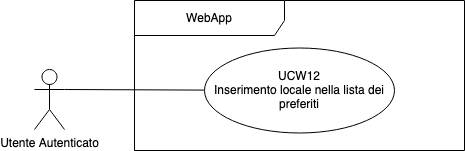
\includegraphics[scale=0.5]{UC_images/UCW12.png} 
    \caption{UCW12 - Inserimento locale nella lista dei preferiti}
\end{figure}
\begin{itemize}
    \item \textbf{Descrizione}: L'utente autenticato inserisce un locale nella lista dei preferiti.
    \item \textbf{Attore primario}: Utente autenticato.
    \item \textbf{Precondizione}: L'utente è autenticato e si trova all’interno della piattaforma Sweeat.
    \item \textbf{Postcondizione}: Viene inserito il locale scelto dall’utente nella lista dei locali preferiti.
    \item \textbf{Scenario principale}: L’utente seleziona dalla lista dei locali il locale da inserire nella lista dei locali preferiti, cliccando su “Aggiungi ai Preferiti”.
\end{itemize}

\subsection{UCW13 - Rimozione locale dalla lista dei preferiti}
\begin{figure}[!h]
\centering
    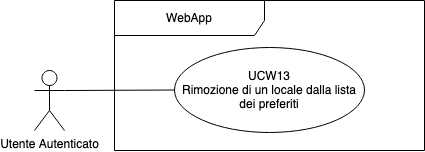
\includegraphics[scale=0.5]{UC_images/UCW13.png} 
    \caption{UCW13 - Rimozione locale dalla lista dei preferiti}
\end{figure}
\begin{itemize}
	\item \textbf{Descrizione}: L'utente autenticato rimuove un locale nella lista dei preferiti.
    \item \textbf{Attore primario}: Utente autenticato.
    \item \textbf{Precondizione}:  L’utente è autenticato nel sistema e c'è almeno un locale inserito nella lista dei locali preferiti dall’utente.
    \item \textbf{Postcondizione}: Viene rimosso il locale scelto dall’utente dalla lista dei locali preferiti.
    \item \textbf{Scenario principale}:
    \begin{enumerate}
        \item L’utente seleziona dalla lista dei locali preferiti il locale da rimuovere dalla lista dei locali preferiti;
        \item L’utente rimuove il locale da rimuovere dalla lista dei locali preferiti, cliccando su “Rimuovi dai Preferiti”.
    \end{enumerate}
\end{itemize}

\pagebreak